%
% Copyright (c) 2011-2012, fortiss GmbH.
% Licensed under the Apache License, Version 2.0.
% 
% Use, modification and distribution are subject to the terms specified
% in the accompanying license file LICENSE.txt located at the root directory
% of this software distribution. A copy is available at
% http://chromosome.fortiss.org/.
%
% This file is part of CHROMOSOME.
%
% $Id$
%
% Author:
%         Dominik Sojer <sojer@fortiss.org>
%         Michael Geisinger <geisinger@fortiss.org>
%

\section{Example 1: Hello World! (20 minutes)}
\label{sec:example_helloworld}

Two steps are required to build an application based on \xme:
the build system has to be generated using CMake and the application needs to be compiled to binary code.
%In \xme, a different build system tree is generated for every single target node in the network.
%This tutorial will only present how CMake can be used to generate the build system for a Windows-based host system.

After the installation of CMake and Visual Studio, the following steps are required:

\begin{enumerate}
	\item Download the Windows release archive of \xme from the website.\footnote{\xme: \url{http://chromosome.fortiss.org/}}
	\item Extract the archive to a directory of your choice (compare Figure~\ref{fig:xme_extracted}).\footnote{%
		Please ensure that the path name is not extraordinary long, as this could cause issues with the build system.}
		After extraction, the subdirectory \verb|src| contains the source code for \xme.
		From now on, we will call that directory \verb|<XME_ROOT>|.
		The subdirectory \verb|bin| contains binaries shipped with the release.
		This allows testing of \xme without compiling your own applications.

\begin{figure}[htpb]
	\centering
	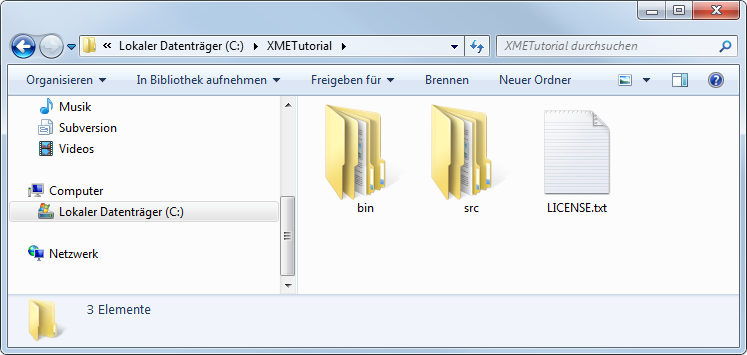
\includegraphics[scale=0.75]{figures/PNG/extracted2.png}
	\caption{Files and folders extracted from the source archive.}
	\label{fig:xme_extracted}
\end{figure}

	\item Use the \emph{start menu} to run \emph{CMake (cmake-gui)} (compare Figure~\ref{fig:cmake_run}).
	\item In the \emph{Where is the source code} field, select the full path to the directory
		\verb|<XME_ROOT>/| \verb|examples/tutorial| (compare Figure~\ref{fig:cmake_configuration1}).

\begin{figure}[htpb]
	\centering
	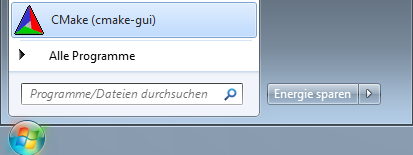
\includegraphics[scale=0.75]{figures/PNG/cmake_run.png}
	\caption{\emph{CMake (cmake-gui)} icon in the start menu.}
	\label{fig:cmake_run}
\end{figure}

\begin{figure}[htpb]
	\centering
	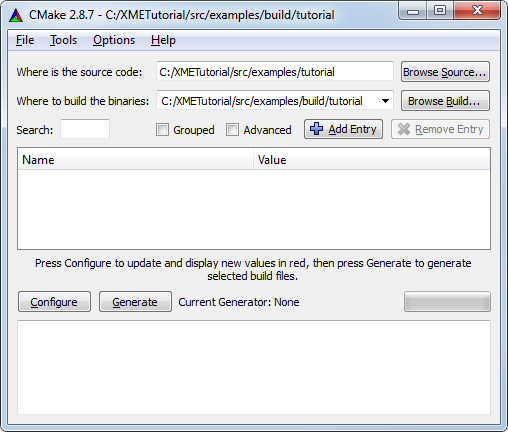
\includegraphics[scale=0.75]{figures/PNG/cmake_configuration1.png}
	\caption{Source code and build directory specification.}
	\label{fig:cmake_configuration1}
\end{figure}

	\item In the \emph{Where to build the binaries} field, select the full path to the directory
		\verb|<XME_ROOT>/| \verb|examples/build/tutorial| (note the additional \verb|build| folder,
		this folder does not yet exist).%\footnote{%
		%This will cause CMake to generate a so-called out-of-source build system, which is recommended.}
	\item Click the \emph{Configure} button.
	\item Choose the \emph{Visual Studio} toolchain that corresponds to your Visual Studio version
		(do \emph{not} use the 64 bit version) and click \emph{Finish} (compare Figure~\ref{fig:cmake_toolchain}).

\begin{figure}[htpb]
	\centering
	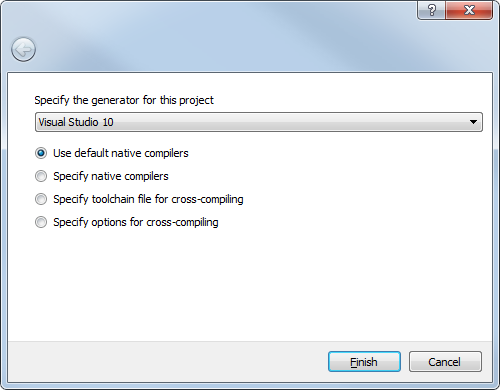
\includegraphics[scale=0.75]{figures/PNG/cmake_toolchain.png}
	\caption{Toolchain selection in CMake.}
	\label{fig:cmake_toolchain}
\end{figure}

	\item After CMake has finished its configuration, various configuration variables marked in red should appear in the list
		(compare Figure~\ref{fig:cmake_configuration2}).
	\item Click the \emph{Generate} button.
		This will generate the Visual Studio solution file \verb|Tutorial.sln| which you can open in Visual Studio.
		The file will be placed in the following directory: \verb|<XME_ROOT>/examples/build/tutorial| (compare Figure~\ref{fig:build_directory}).

\begin{figure}[h!t]
	\centering
	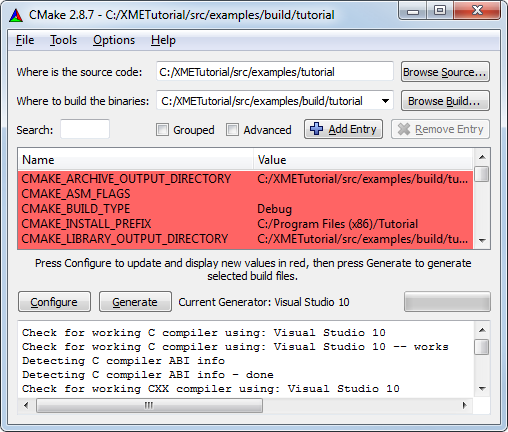
\includegraphics[scale=0.75]{figures/PNG/cmake_configuration2.png}
	\caption{Configuration and build system generation in CMake.}
	\label{fig:cmake_configuration2}
\end{figure}

\begin{figure}[htpb]
	\centering
	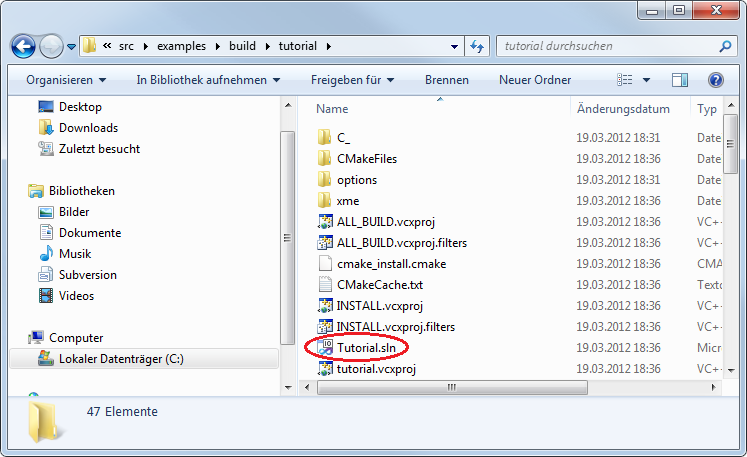
\includegraphics[scale=0.75]{figures/PNG/build_directory_edited.png}
	\caption{Build directory after build system generation, highlighted in red the Visual Studio solution file.}
	\label{fig:build_directory}
\end{figure}

\end{enumerate}

\noindent To compile the exemplified application, the following steps are required:

\begin{enumerate}
	\item Fire up Visual Studio and select \emph{File} $\rightarrow$ \emph{Open} $\rightarrow$ \emph{Project/Solution...}
	\item Navigate to the \verb|<XME_ROOT>/examples/build/tutorial| directory and select the solution file \verb|Tutorial.sln|.
	\item After loading the solution, you will see a project tree in the left-hand pane.
		Right-click on the \verb|tutorial| project and choose \emph{Set as StartUp Project}
		(compare Figure~\ref{fig:vs_set_as_startup_project}).

\begin{figure}[htpb]
	\centering
	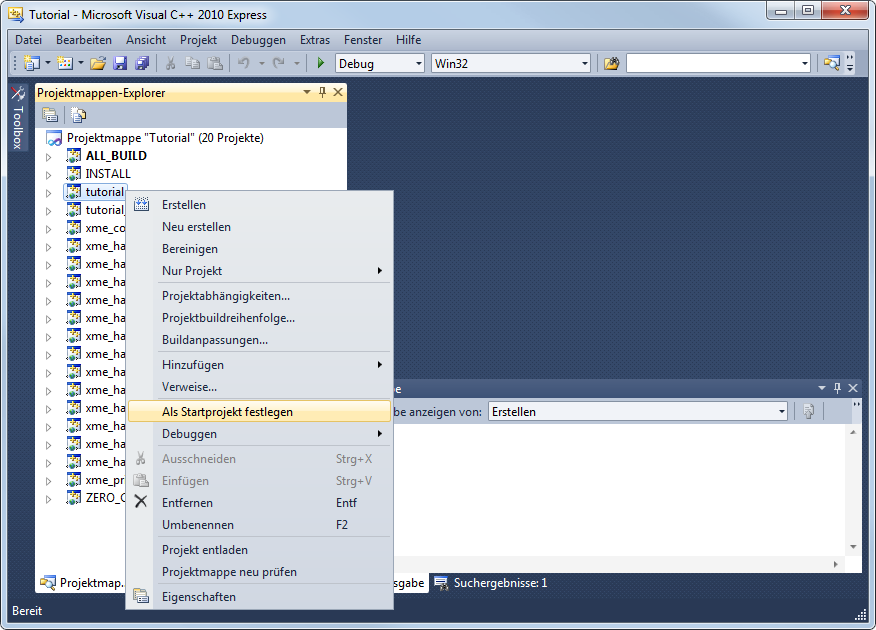
\includegraphics[scale=0.5]{figures/PNG/vs_set_as_startup_project.png}
	\caption{Setting the \texttt{tutorial} project as \emph{StartUp Project}.}
	\label{fig:vs_set_as_startup_project}
\end{figure}

	\item In the tool bar, select the solution configuration you want to build (usually \texttt{Debug} or \texttt{Release}).
		The \texttt{Debug} build includes debugging information and should be used for development.
		If in doubt, choose \texttt{Release}.

	\item Hit \emph{F7} to compile the solution.

	\item Debug/run the project as usual (e.g., hit \emph{F5} to debug or \emph{Ctrl+F5} to run without debugging).
		If you get prompted whether to rebuild the out-of-date \texttt{ZERO\_CHECK} project (compare Figure~\ref{fig:vs_zero_check}),
		you may select the \emph{Do not show this dialog box again} check box and choose \emph{Yes}.

	\item When the application starts, you will probably receive a query from the \emph{Windows Firewall}.
		\xme is designed to talk to other nodes in the network and hence needs a firewall exception for full functionality.
		If you do not want the \xme to talk to other nodes, then simply deny access.\footnote{%
		If you want to allow access to the network at a later point in time,
		you can change the Firewall settings in the \emph{System Control Panel}.}
		In this case, communication will be limited to \xme applications on the local computer.
		If you want \xme applications to communicate with each other in the local network,
		allow access to the \emph{Home or Company Network} as shown in Figure~\ref{fig:firewall_tutorial}.

\begin{figure}[htpb]
	\centering
	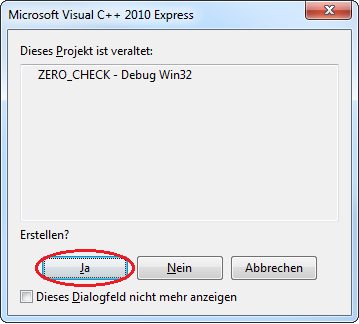
\includegraphics[scale=0.75]{figures/PNG/vs_zero_check_edited.png}
	\caption{\texttt{ZERO\_CHECK} project out of date prompt.}
	\label{fig:vs_zero_check}
\end{figure}

\begin{figure}[htpb]
	\centering
	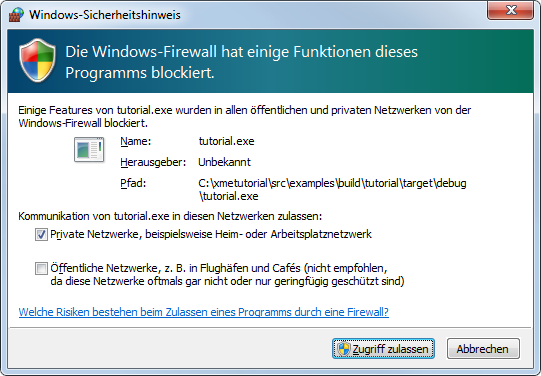
\includegraphics[scale=0.75]{figures/PNG/firewall_tutorial.png}
	\caption{Firewall settings for the \texttt{Tutorial} application.}
	\label{fig:firewall_tutorial}
\end{figure}

\end{enumerate}

This tutorial is bundled with a simple \emph{Hello World} example application, which gets built when this workflow is executed.
The entry point into the executable is in \verb|tutorial.c|, which also defines the \xme components used in this application.
The application is composed of some software components that are explained in section \ref{sec:core_components}
(\emph{Node Manager}, \emph{IP Login Server Proxy}) and an application-specific components called \emph{Hello World Component}).
The latter one prints the text ``\texttt{Hello World!}'' to the console every two seconds (compare Figure~\ref{fig:example_hello_world}).
%
You may now inspect the source code in the files \verb|tutorial.c|, \verb|helloWorldComponent.c| and \verb|helloWorldComponent.h|
to see how the concepts from Section~\ref{sec:architecture} are used in the application.

\begin{figure}[htpb]
	\centering
	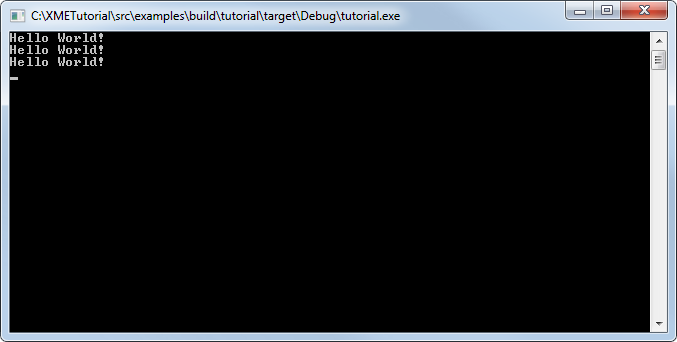
\includegraphics[scale=0.75]{figures/PNG/example_hello_world.png}
	\caption{\emph{Hello World Component} printing messages to the console.}
	\label{fig:example_hello_world}
\end{figure}
